\documentclass{article}

\usepackage{fancyhdr}
\usepackage{extramarks}
\usepackage{amsmath}
\usepackage{amsthm}
\usepackage{amsfonts}
\usepackage{tikz}
\usetikzlibrary{calc,arrows}
\usepackage[plain]{algorithm}
\usepackage{algpseudocode}
\usepackage{enumitem} %% for custom list
\usepackage{graphicx} %% used to split page in two columns
\usepackage{multicol}
\usetikzlibrary{automata,positioning}

\usepackage{mathtools}
\DeclarePairedDelimiter\ceil{\lceil}{\rceil}
\DeclarePairedDelimiter\floor{\lfloor}{\rfloor}

% using \code{come code monospaced}
\def\code#1{\texttt{#1}}

%
% Basic Document Settings
\topmargin=-0.45in
\evensidemargin=0in
\oddsidemargin=0in
\textwidth=6.5in
\textheight=9.0in
\headsep=0.25in

\linespread{1.1}

\pagestyle{fancy}
\lfoot{\lastxmark}
\cfoot{\thepage}

\renewcommand\headrulewidth{0.4pt}
\renewcommand\footrulewidth{0.4pt}

\setlength\parindent{0pt}

\setcounter{secnumdepth}{0}

% change name of the problem here
\newenvironment{homeworkProblem}[1][-1]{
    \section{TCP}
}{}
\nobreak\extramarks{TCP}{}\nobreak{}


\begin{document}

\begin{homeworkProblem}
	Si deve effettuare un trasferimento \code{HTTP} di un file di 16300 byte, si assuma che il comando \code{PUT} occupi 300 
	byte. Il tempo di propagazione \(T_p\) \'e di 1 ms.
	La velocit\'a di trasmissione a livello IP \'e di 4800000 bit/s = 4.8 Mbps. Le due entit\'a si trovano su due sottoreti 
	diverse, separati da un router.

    \begin{enumerate}[noitemsep]
        \item La consegna dei datagrammi IP avviene in modo diretto o indiretto ?
        \item Che valore assume la MSS di TCP in assenza di opzioni e con normale header IP ?
        \item Si mostrino i segmenti scambiati per l'apertura della connessione TCP conseguente al comando \code{PUT}.
        \item Che dimensione ha l'ultimo segmento della connessione ?
        \item Si mostri l'intero scambio dei pacchetti TCP per il trasferimento del file incluso lo scambio finale per la 
              chiusura della connessione. Si calcoli il tempo di trasferimento.
        \item Si mostri l'intero scambio dei pacchetti TCP per il trasferimento del file nel caso si perda il \(4^o\) e il 
              \(9^o\) segmento con RTO = 120 ms.
        \item Che costo ha avuto in termini di efficienza della trasmissione aver perso questi pacchetti ?
    \end{enumerate}

    \textbf{1)}
    La consegna avviene in modo indiretto perch\'e i due host si trovano in sottoreti diverse.
    \\

    \textbf{2)}
    Essendo che stiamo parlando di una rete cablata Ethernet possiamo dire che:
    \[
        \begin{split}
            \text{MTU} &= 1500\ \text{bytes}
            \\
            \text{MSS} &= \text{MTU} - \text{header IP} - \text{header TCP} =
            \\
            &= 1500\ \text{byte} - 20\ \text{byte} - 20\ \text{byte} =
            \\
            &= 1460\ \text{byte}
        \end{split}
    \]
    \\

    \textbf{3)}
    \begin{multicols}{2}[\columnsep4em] 	
		\[
			\begin{split}
            	\text{Porta Server} =&\ 80 \text{, porta HTTP standard}
            	\\
            	\text{Porta Client} =&\ \text{random} > 1024\ \text{ad esempio } 1025
            	\\
            	\text{SQNc} =&\ \text{numero casuale nello spazio di}
           		\\
           		&\text{ numerazione di TCP}
            	\\
            	\text{SQNs} =&\ \text{SQNc} + 1            	
        	\end{split}
		\]
		Nel momento in cui ricevo il \code{SYNACK} dal server la connessione \'e gi\'a aperta da parte del server, quindi 
		\'e gi\'a pronto a ricever i dati.	Si pu\'o quindi assumere che gli \code{ACK} siano inviati in piggybacking sui 
		dati, quindi posso iniziare a trasmettere il file al posto dell'ultimo \code{ACK}.
		
		\columnbreak
	
		\begin{center}
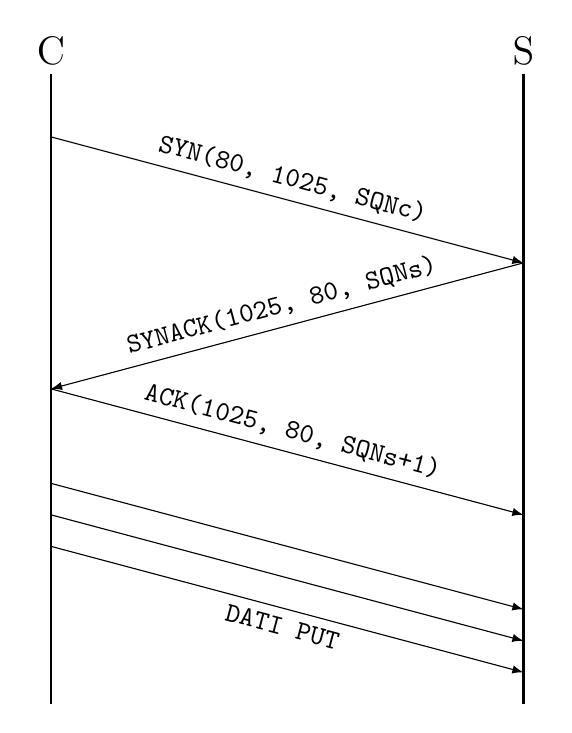
\begin{tikzpicture}[>=latex]

	% define the coordinates of client timeline
	\coordinate (A) at (0,8);
	\coordinate (B) at (0,0);
	
	% defien the coordinates of server timeline
	\coordinate (D) at (6,0);
	\coordinate (C) at (6,8);
	
	% draw client and server timeline
	\draw[thick] (A)--(B) (C)--(D);
	% label it on the top	
	\draw (A) node[above]{\Large C};
	\draw (C) node[above]{\Large S};

	\coordinate (E) at ($(A)!.1!(B)$);
	\draw (E) node[left]{
		\begin{tabular}{r}
			%\textit{}\\
			%\verb$$
		\end{tabular}
	};

	\coordinate (F) at ($(C)!.3!(D)$);
	\draw (F) node[right]{
		\begin{tabular}{l}
			%\verb$$\\
			%textit{}
		\end{tabular}
	};	
	\draw[->] (E) -- (F) node[midway,sloped,above]{\verb$SYN(80, 1025, SQNc)$};

	\coordinate (G) at ($(A)!.5!(B)$);
	\coordinate (G1) at ($(A)!.65!(B)$);
	\coordinate (G2) at ($(A)!.70!(B)$);
	\coordinate (G3) at ($(A)!.75!(B)$);
	\draw (G) node[left]{
		\begin{tabular}{l}
			%\verb$$
		\end{tabular}
	};
	\draw[->] (F) -- (G) node[midway,sloped,above]{\verb$SYNACK(1025, 80, SQNs)$};

	\coordinate (H) at ($(C)!.7!(D)$);
	\coordinate (H1) at ($(C)!.85!(D)$);
	\coordinate (H2) at ($(C)!.90!(D)$);
	\coordinate (H3) at ($(C)!.95!(D)$);
	\draw (H) node[right]{
		\begin{tabular}{l}
			%\verb$$
		\end{tabular}
	};
	\draw[->] (G) -- (H) node[midway,sloped,above]{\verb$ACK(1025, 80, SQNs+1)$};
	
	\draw[->] (G1) -- (H1) node[midway,sloped,above]{\verb$$};
	\draw[->] (G2) -- (H2) node[midway,sloped,above]{\verb$$};
	\draw[->] (G3) -- (H3) node[midway,sloped,below]{\verb$DATI PUT$};	
	
\end{tikzpicture}
\end{center}

	\end{multicols}    
    
    \pagebreak
    \textbf{4)} 
    Il numero di segmenti necessari al trasferimento del file sono:
    \[
    	N_{segm}\ =\ \ceil*{\frac{\text{dimensione file}}{\text{MSS}}}
    	=\ \ceil*{\frac{16300\ \text{byte}}{1460\ \text{byte}}} =\ 12
    \]
    Ora trovo la lunghezza dell'ultimo segmento
    \[
    	16300\ \text{byte} - (12-1) \cdot 1460\ \text{byte} = 240\ \text{byte}
    \]
    \\    
    
    \textbf{5)}
    Il tempo di trasmissione di un datagramma IP \'e pari a
    \[
    	\begin{split}
    		T_{tx} =&\ \frac{1500\ \text{byte} \cdot 8}{4.8\ \text{Mbps}}
    		=\ \frac{12000\ \text{bit}}{4.8 \cdot 10^6\ \text{bps}}
    		=\ 2.5 \cdot 10^{-3}\ \text{s} =\ 2.5\ \text{ms}
    	\end{split}
    \]
    Mentre l'ultimo segmento, essendo di dimensioni minori, impiegher\'a
    \[
    	\begin{split}
    		T_{tx}N =&\ \frac{(240\ \text{byte} + 20 \cdot 2\ \text{byte}) \cdot 8}{4.8\ \text{Mbps}}
    		=\ \frac{2240\ \text{bit}}{4.8 \cdot 10^6\ \text{bps}}
    		=\ 4.6 \cdot 10^{-4}\ \text{s}\ =\ 0.46\ \text{ms}
    	\end{split}
    \]
    Ai \(240\) byte dell'ultimo segmento vanno aggiunti i \(40\) byte di header IP e TCP. Nel calcolo di \(T_{tx}\) non
    vengono aggiunti perch\'e ho usato la MTU Ethernet. Il tempo totale di trasmissione senza perdite \'e quindi di
    \[
    	\begin{split}
    		T_{tx}tot =&\ 11 \cdot T_{tx} + T_{tx}N = 11 \cdot 2.5\ \text{ms} + 0.46\ \text{ms} = 27.96\ \text{ms}
    	\end{split}
    \]
    
    \pagebreak
    \textbf{6)}
    
    \pagebreak
    \textbf{7)}
    L'efficienza senza perdite \'e data da
    \[
    	\begin{split}
    		U_w\ =\ \frac{N_{segm} \cdot T_{tx}tot}{2 \cdot T_{p} + T_{tx}tot}
    		=\ \frac{12 \cdot 27.96\ \text{ms}}{2\ \text{ms} + 27.96\ \text{ms}}
    		=\ \frac{335.52\ \text{ms}}{29.96\ \text{ms}}
    		=\ 11.19
    	\end{split}
    \]
   	\\
   	Il tempo di trasmissione nel caso di perdite \'e dominato dal RTO, quindi l'efficienza risulta
   	\[
    	\begin{split}
    		U_p\ =\ \frac{N_{segm} \cdot T_{tx}tot}{\approx RTO}
    		=\ \frac{12 \cdot 27.96\ \text{ms}}{\approx120\ \text{ms}}
    		=\ \frac{335.52\ \text{ms}}{\approx 120\ \text{ms}}
    		=\ 2.796
    	\end{split}
    \]
    Con una perdita di efficienza nell'ordine del
    \[
    	\begin{split}
    		\frac{U_p}{U_w} \cdot 100\ =\ 25\ \%
    	\end{split}
    \]

\end{homeworkProblem}

\end{document}
